\begin{figure}[htp]
	\centering
	\subfloat[Data]
	{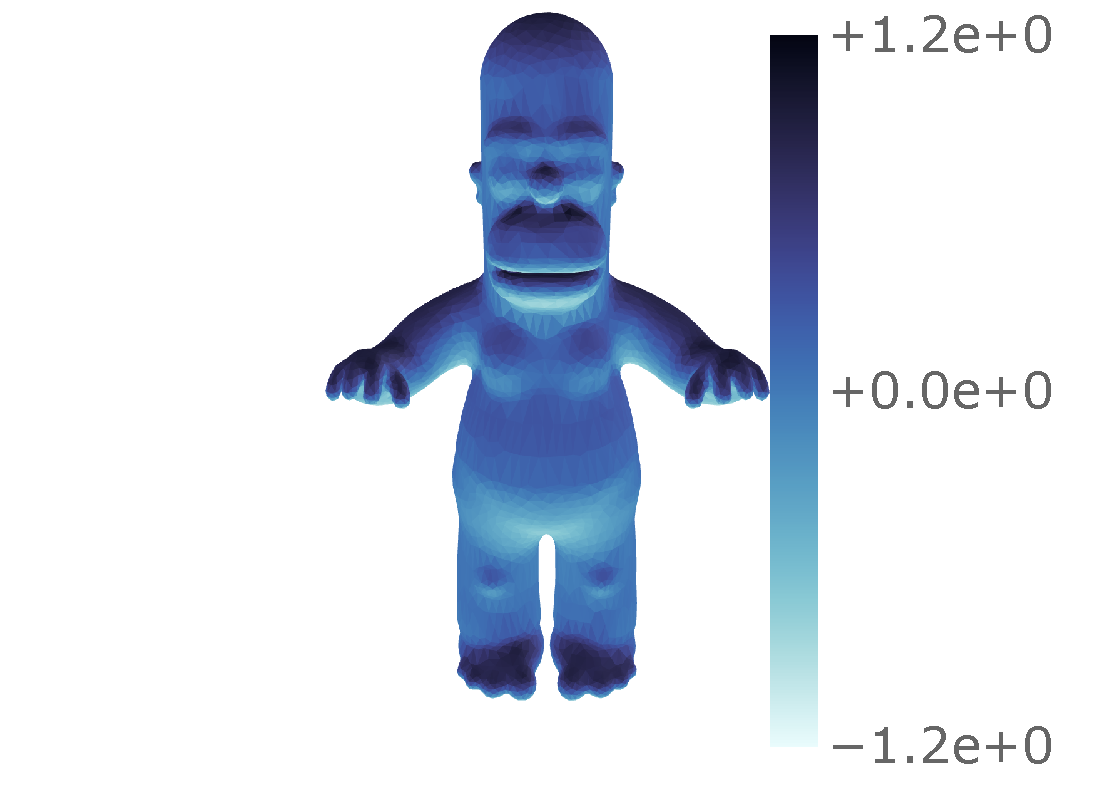
\includegraphics[trim={156 8 21 6},clip,width=.46\textwidth]{homer_field.pdf}}
	\hfill
	\subfloat[\(R\)]
	{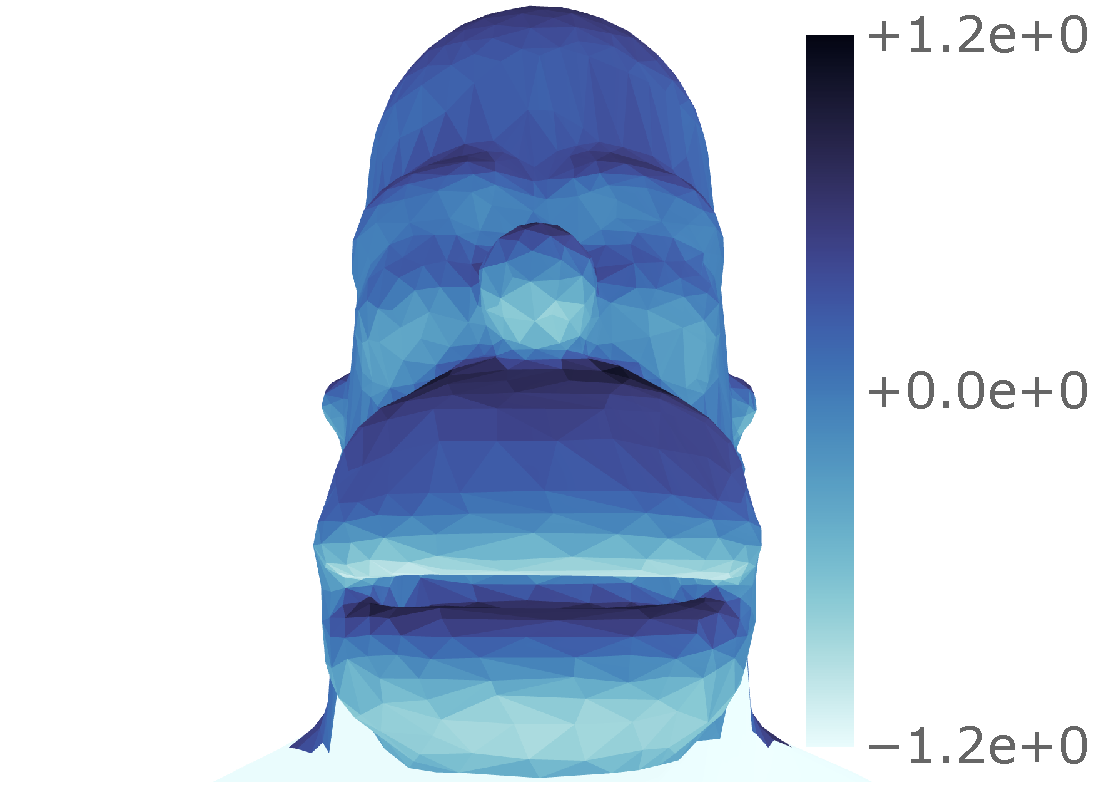
\includegraphics[trim={101 0 3 3},clip,width=.54\textwidth]{slepian_homer_field_zoom.pdf}}
	\caption{
		Panel (a) corresponds to the z-component of the per vertex normals of the Homer mesh.
		Panel (b) presents the region \(R\), which is constructed from Slepian coefficients of the Homer head region.
		The field value outside the region in panel (b) is set to negative infinity for illustrative purposes.
	}\label{fig:chapter4_homer_data}
\end{figure}
